% Created 2018-10-02 Tue 01:53
% Intended LaTeX compiler: pdflatex
\documentclass[10pt,t]{beamer}
\usepackage[utf8]{inputenc}
\usepackage[T1]{fontenc}
\usepackage{graphicx}
\usepackage{grffile}
\usepackage{longtable}
\usepackage{wrapfig}
\usepackage{rotating}
\usepackage[normalem]{ulem}
\usepackage{amsmath}
\usepackage{textcomp}
\usepackage{amssymb}
\usepackage{capt-of}
\usepackage{hyperref}
\usetheme{default}
\author{L. Larrabee Strow}
\date{\today}
\title{\large AIRS Plus CrIS/IASI Multi-Decadal Trends and Anomalies with Full Spatial Sampling and Rigorous Error Characterization}
\subtitle{\footnotesize{AIRS Science Team Meeting}}
\date{\vspace{0.1in}\footnotesize{October 3, 2018 \vfill}}
\author{L. Larrabee Strow\inst{1,2}, Sergio De-Souza Machado\inst{1,2}, Steven Leroy\inst{3}, Howard Motteler\inst{2}, Chris Hepplewhite\inst{2}, and Steven Buczkowski\inst{2}}
\institute[UMBC]{\inst{1} UMBC Physics Dept. \and \inst{2}UMBC JCET \and \inst{3} AER}
\input beamer_setup
\usetheme{metropolis}
\metroset{titleformat title=allcaps}
\renewcommand{\UrlFont}{\small\tt}
\renewcommand*{\UrlFont}{\footnotesize}
\tolerance=1000
\RequirePackage{fancyvrb}
\DefineVerbatimEnvironment{verbatim}{Verbatim}{fontsize=\footnotesize}
\hypersetup{
 pdfauthor={L. Larrabee Strow},
 pdftitle={\large AIRS Plus CrIS/IASI Multi-Decadal Trends and Anomalies with Full Spatial Sampling and Rigorous Error Characterization},
 pdfkeywords={},
 pdfsubject={},
 pdfcreator={Emacs 25.1.1 (Org mode 9.1.12)}, 
 pdflang={English}}
\begin{document}

\maketitle
\addtobeamertemplate{block begin}{
  \setlength{\parsep}{0pt}
  \setlength{\topsep}{3pt plus 2pt minus 2.5pt}
  \setlength{\itemsep}{0pt plus 0pt minus 2pt}
  \setlength{\partopsep}{2pt}
}

\begin{frame}[shrink=20,label={sec:orgc51264c}]{Overview:  Two Products Proposed}
\vspace{-0.1in}
\begin{block}{(1) Multi-Instrument Hyperspectral Radiance Climate Time Series}
\begin{itemize}
\item 1:30 Orbit: AIRS + CrIS, 9:30 Orbit: IASI
\item Convert to common ILS to allows inter-instrument radiance calibration
\item Emphasizes routine/fast processing of data for extensive testing
\item Produce time/space grids of radiance time series and anomalies for climate analysis
\end{itemize}
\end{block}

\begin{block}{(2) Level 3 Geophysical Products}
\begin{itemize}
\item Generate geophysical (T/Q, etc.) "Level 3" anomaly time series and trends from radiance trends and anomailes
\item This approach reduces influence of a-priori and allows better error estimation?
\item May include well established microwave radiance products in retrievals
\end{itemize}
\end{block}

\begin{block}{Validation/Comparisons}
\begin{itemize}
\item Reanalysis: ERA+, MERRA-2
\item Microwave
\item Surface and SST climatologies
\item GPS-RO (Leroy)
\end{itemize}
\end{block}
\end{frame}

\begin{frame}[label={sec:org2419427}]{Time Series Length Nearing Climate Scales}
\vspace{-0.3in}

\begin{columns}
\begin{column}{0.55\columnwidth}
\begin{block}{\footnotesize CLARREO Schematic: Our Uncertainty?}
\begin{center}
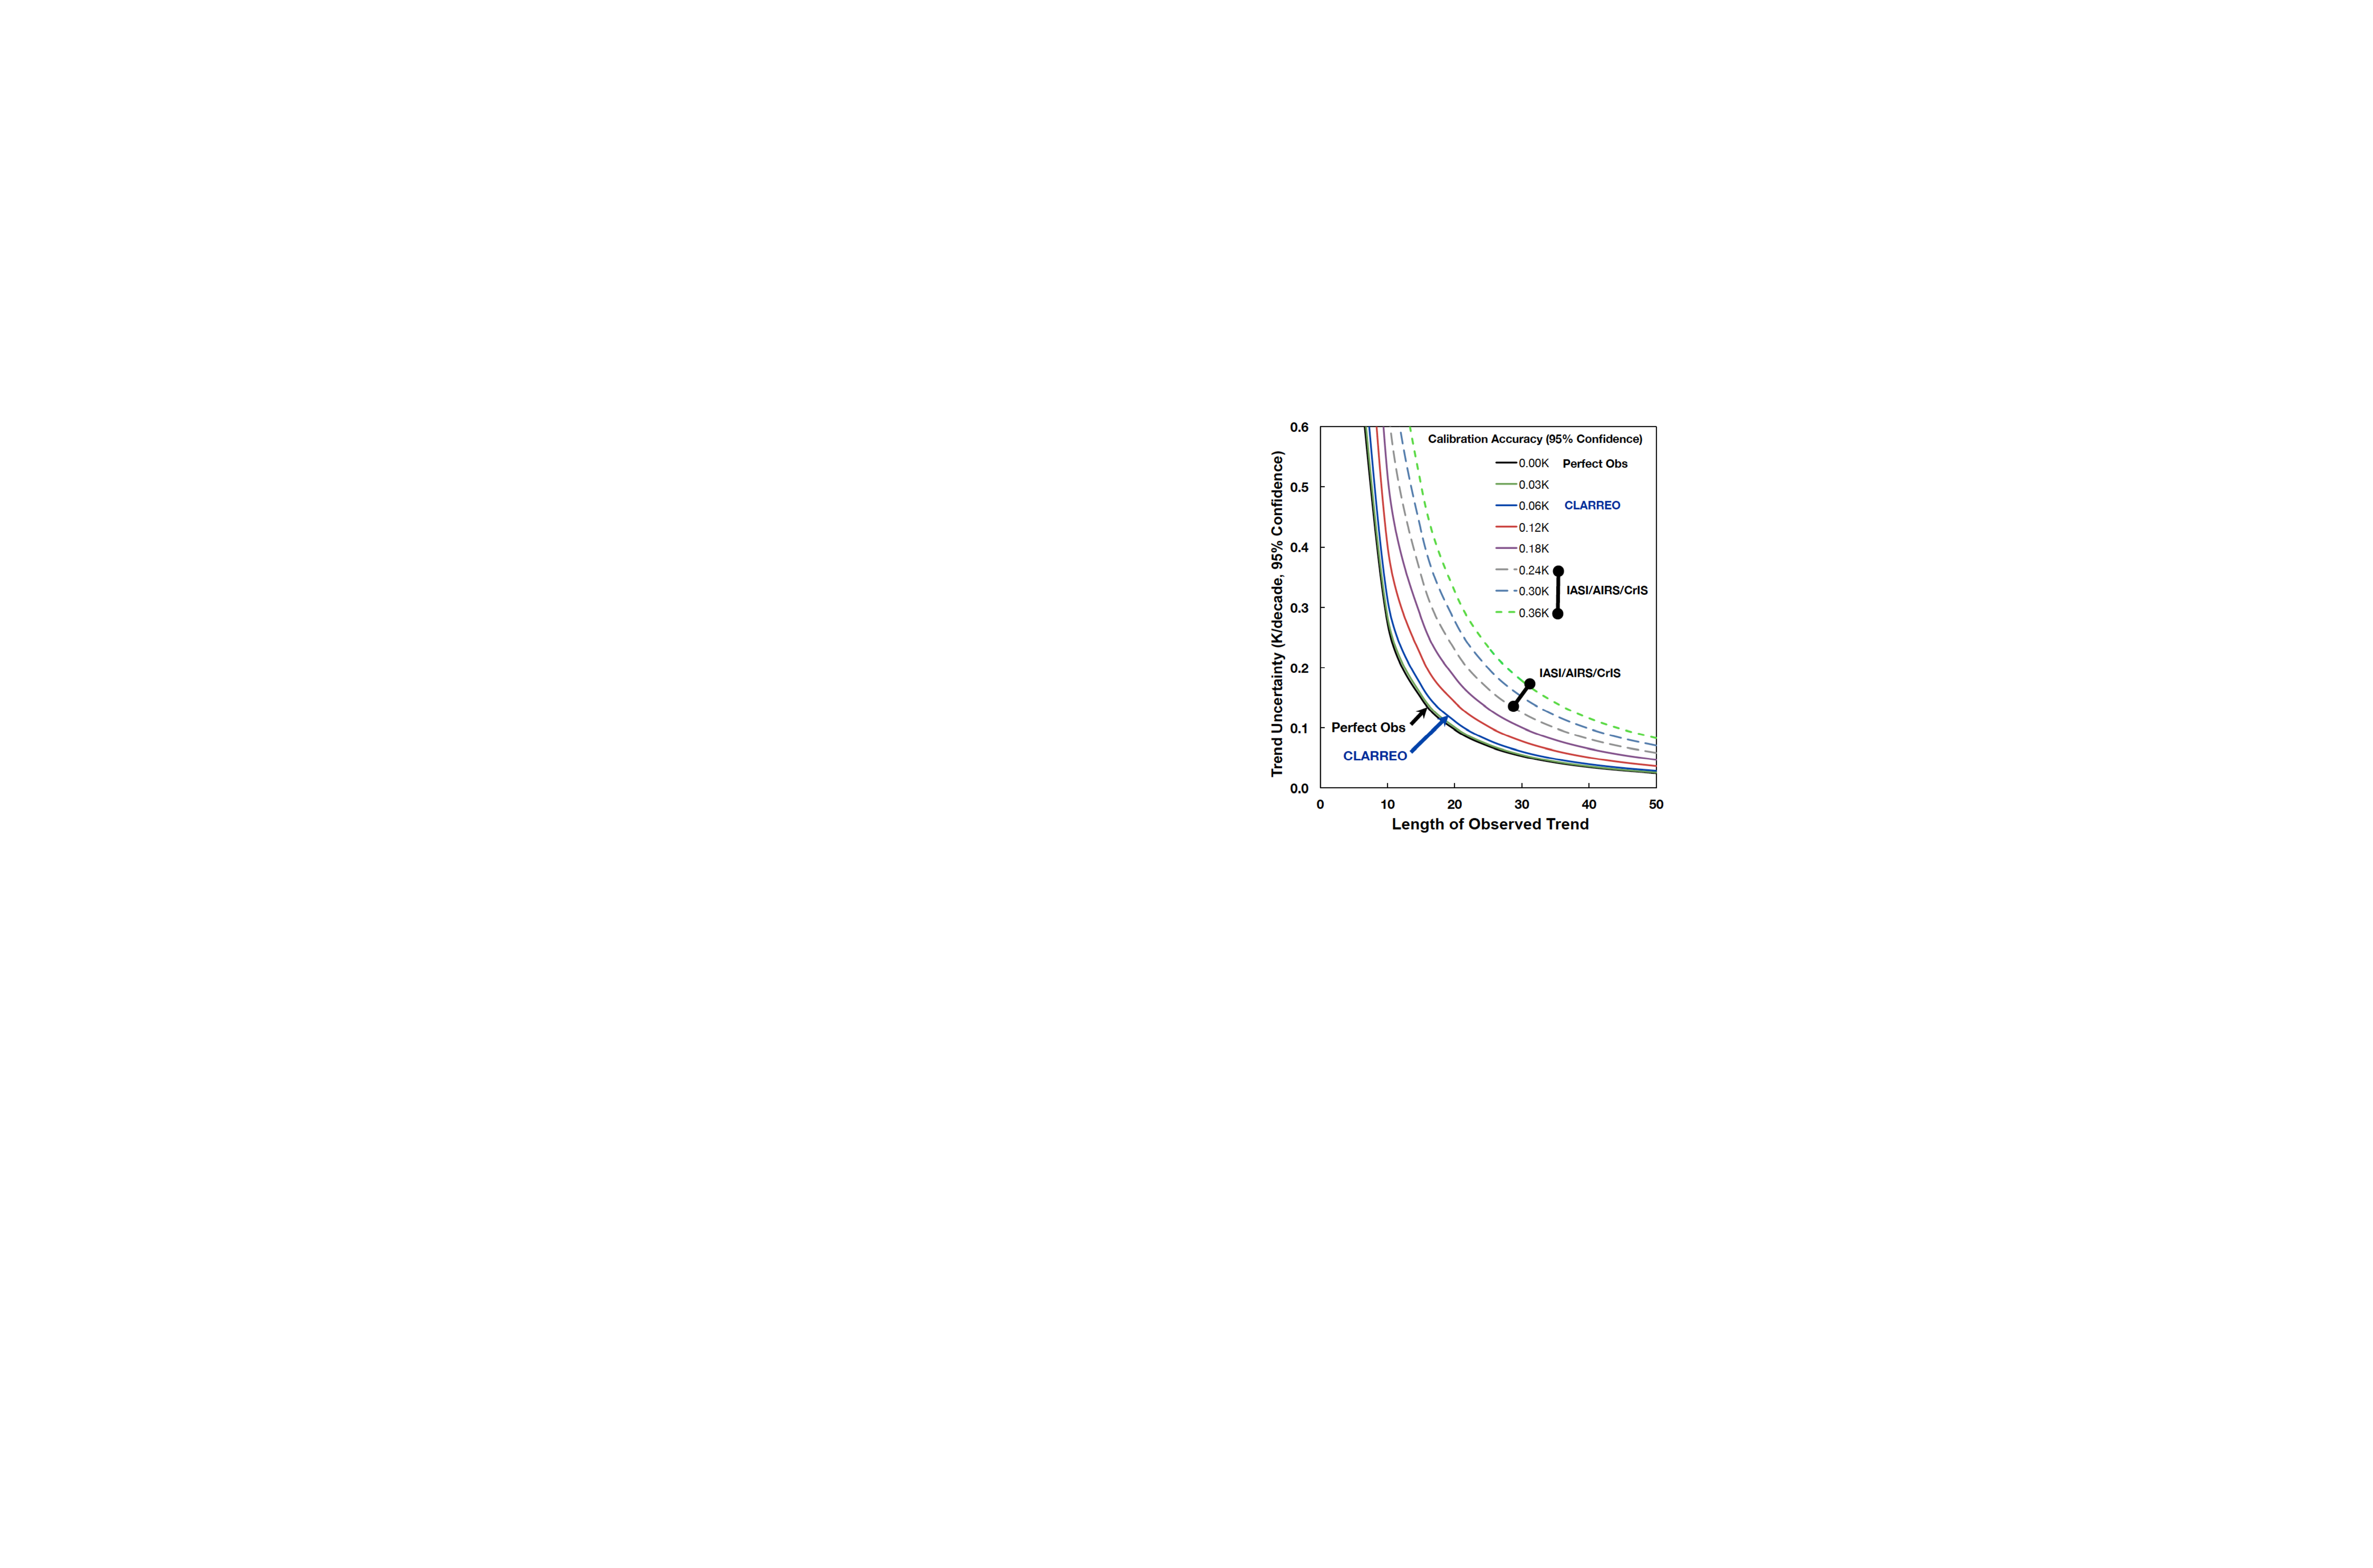
\includegraphics[width=.9\linewidth]{./Figs/Pdf/clarreo.pdf}
\end{center}
\vspace{0.1in}
\footnotesize
AIRS, CrIS, IASI are \emph{all} very stable
\end{block}
\end{column}

\begin{column}{0.55\columnwidth}
\begin{block}{\footnotesize AIRS 14-Year global trends}
\begin{center}
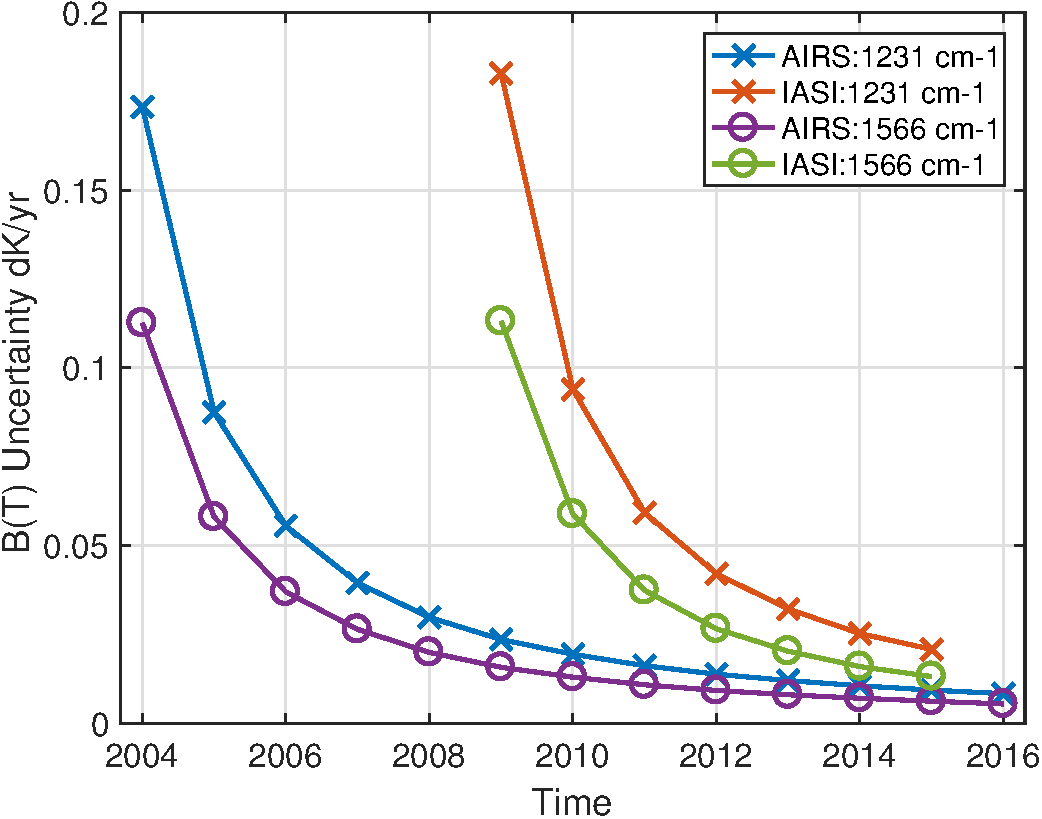
\includegraphics[width=\linewidth]{./Figs/Pdf/1231and1566cm-1_dbt_uncertainty_vs_time_iasi_airs_2016_v2.pdf}
\end{center}

\footnotesize
These are 2-\(\sigma\) B(T) statistical uncertainties due to inter-annual variability.  

Some channels, some latitudes not gaussian (strat sudden warmings, QBO, etc.)
\end{block}
\end{column}
\end{columns}
\end{frame}

\begin{frame}[label={sec:org5837a87}]{CHIRB Processing Flow}
\vspace{-0.2in}
\begin{center}
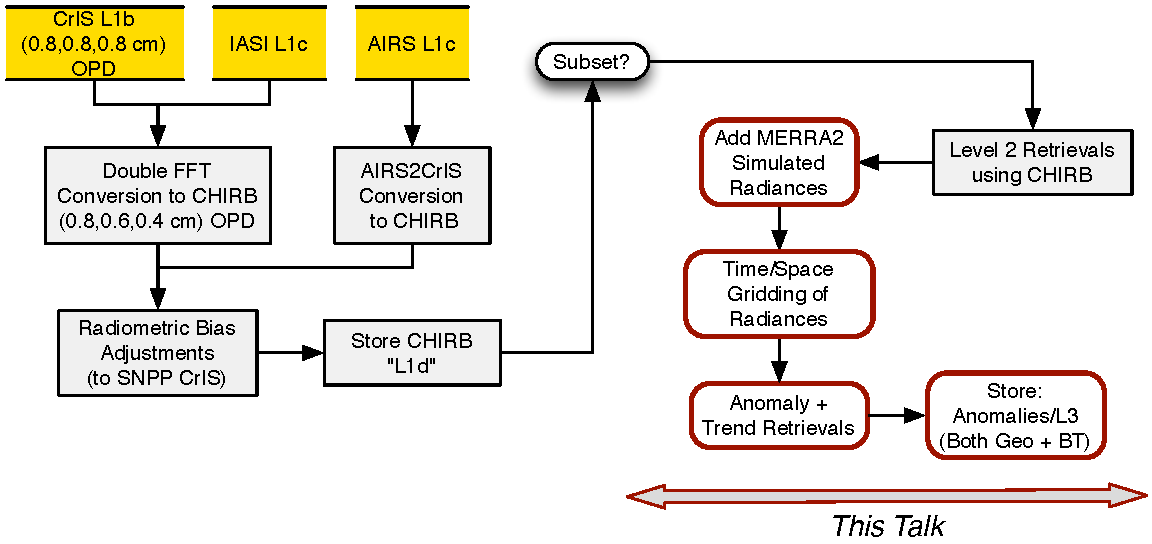
\includegraphics[width=1.0\linewidth]{./airs2cris_stm_talk2_landscape.pdf}
\end{center}

CHIRB: (Common or Climate) Hyperspectral InfraRed Basis

0.8 /0.6 /04  

0.0625 / 0.0833  /  0.1250
\end{frame}

\begin{frame}[label={sec:orga6ca73e}]{Time/Space Gridded Radiance Data Flow}
\vspace{-0.1in}
\begin{center}
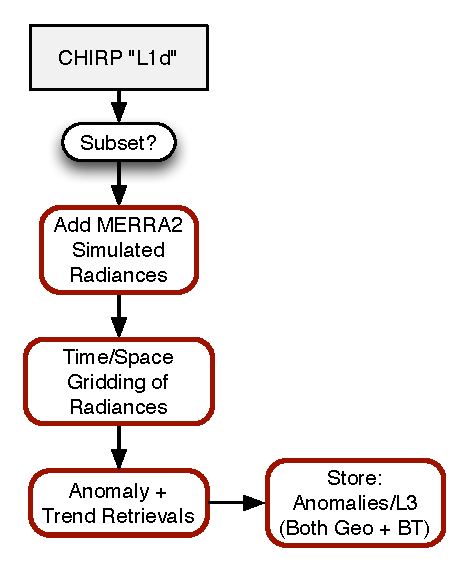
\includegraphics[width=0.6\linewidth]{./airs2cris_stm_talk2_small.pdf}
\end{center}
\end{frame}

\begin{frame}[label={sec:org5dfe0c4}]{Anomaly and Trend Approach}
Linear solution for trends with a-priori state = 0 given by,
\begin{displaymath}
\frac{dx}{dt} =  \left(K^T S_{\epsilon}^{-1} K + R^{-1}\right)^{-1} \left(K^T S_{\epsilon}^{-1} \frac{dBT}{dt}\right)
\end{displaymath}

\begin{itemize}
\item \emph{x} is the atmospheric state
\item \emph{K} are the B(T) Jacobians
\item \(S_{\epsilon}\) is the observation error covariance matrix.
\item \emph{R} combines empirical regularization (Tikonov L1-type) and the \emph{a-priori} covariance-based terms
\end{itemize}

\(S_\epsilon\) covariances represent inter-annual variability and instrument stability.  Provides signficiant constraints compared to L3 time derivatives.

Jacobian state from standard all-sky retrievals or from re-analysis; high accuracy not needed.
\end{frame}

\begin{frame}[shrink=20,label={sec:org93c6f91}]{MERRA2, ERA, etc}
\begin{itemize}
\item Barnet's CLIMCAPS will use MERRA-2 as a-priori
\item My understanding is that MERRA-2 will be embedded in the CLIMAPS products
\end{itemize}

\begin{block}{This Work}
\begin{itemize}
\item We match every radiance measurement with ERA (and soon MERRA-2)
\item We simulated radiances from MERRA-2 and use them to test our retrieval algorithms
\item Our Jacobians are dependent on MERRA-2 profiles
\item MERRA-2 also provides partial validation
\end{itemize}
\end{block}

\begin{block}{Suggestion}
\begin{itemize}
\item Create a separate Sounding Product that co-locates MERRA-2 with each observation
\item Provides a common resource for our sounding algorithms and for future users
\item Maybe we could get MERRA-2 integrated to the sensor observation time (w/in 1/2 hour instead of 3 hours)?
\end{itemize}
\end{block}
\end{frame}

\begin{frame}[label={sec:orge052ea3}]{Data Used for Preliminary Results}
\begin{itemize}
\item Start with a \textasciitilde{}1\% random, area-weighted subset (for quick processing)
\item Produce 40 area weighted zonal bins
\item Save daily averages of these 40 zonal bins
\end{itemize}

Long-term: 16 day bins using 3x5 degree grids derived from all data (not from just 1\% random subset)

\begin{block}{Data set size for preliminary work:}
\begin{itemize}
\item (5475 days) X (2645 L1c spectral channels) X (40 latitude bins)
\end{itemize}
\end{block}
\end{frame}

\begin{frame}[label={sec:orgf6b0bcd}]{Global B(T) Trend (Area Weighted)}
\vspace{-0.15in}
\begin{center}
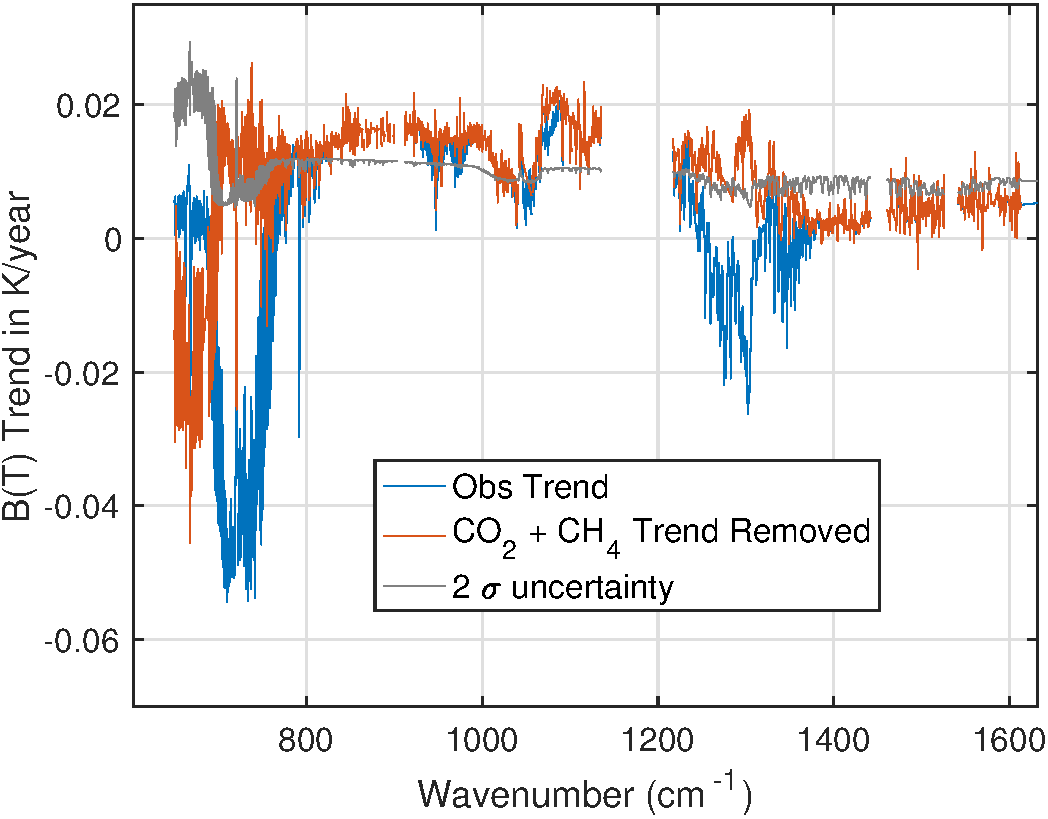
\includegraphics[width=0.7\linewidth]{./oFigs/airs_14year_global_trends.pdf}
\end{center}

\small
\begin{itemize}
\item \cd corrected trends show nominal 0.015K/year warming for the surface and throughout the troposphere
\item \cd corrected stratospheric channels show cooling
\end{itemize}
\end{frame}

\begin{frame}[label={sec:org467c2c2}]{Retrieved Zonal Trends (T/\water/T\(_{\text{surf}}\))}
\vspace{-0.35in}

\begin{columns}
\begin{column}{0.55\columnwidth}
\begin{block}{\footnotesize Temperature (K/Decade)}
\vspace{-0.1in}
\begin{center}
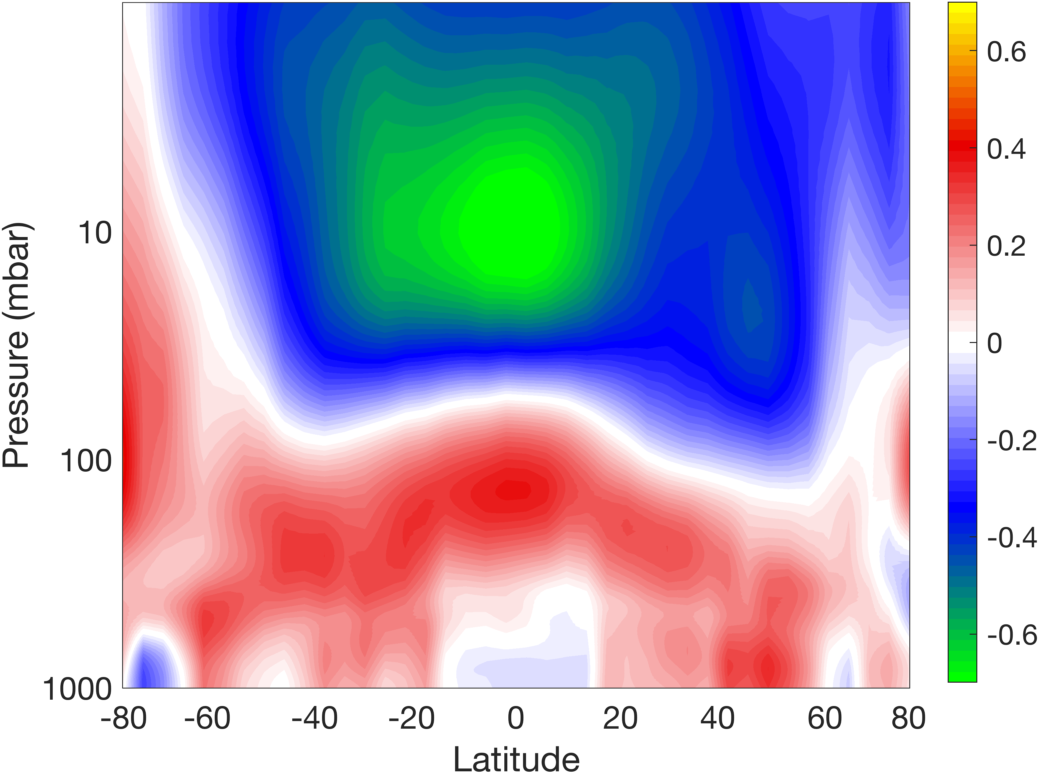
\includegraphics[width=0.8\linewidth]{./Figs/Png/temp_trend.png}
\end{center}
\end{block}
\end{column}

\begin{column}{0.55\columnwidth}
\begin{block}{\footnotesize Water Vapor (\%/Year)}
\vspace{-0.1in}
\begin{center}
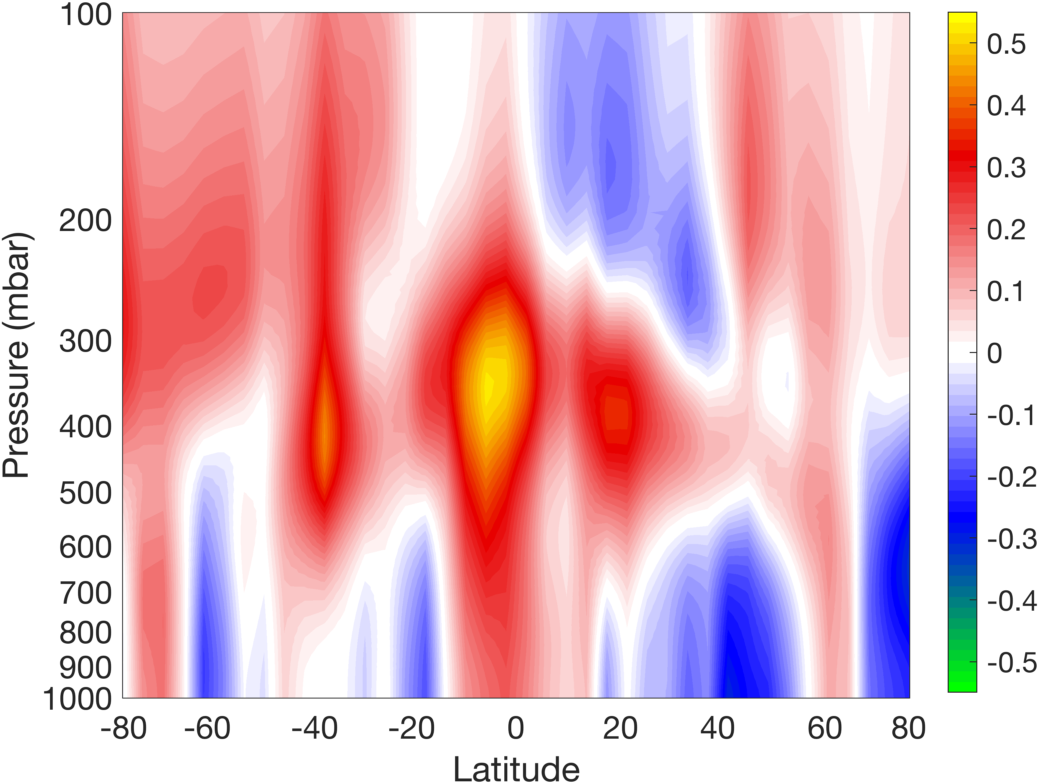
\includegraphics[width=0.8\linewidth]{./Figs/Png/wat_trend.png}
\end{center}
\end{block}
\end{column}
\end{columns}

\vspace{-0.2in}
\begin{columns}
\begin{column}{0.55\columnwidth}
\begin{block}{\footnotesize Surface Temperature (K/Decade)}
\vspace{-0.05in}
\vspace{-0.05in}
\begin{center}
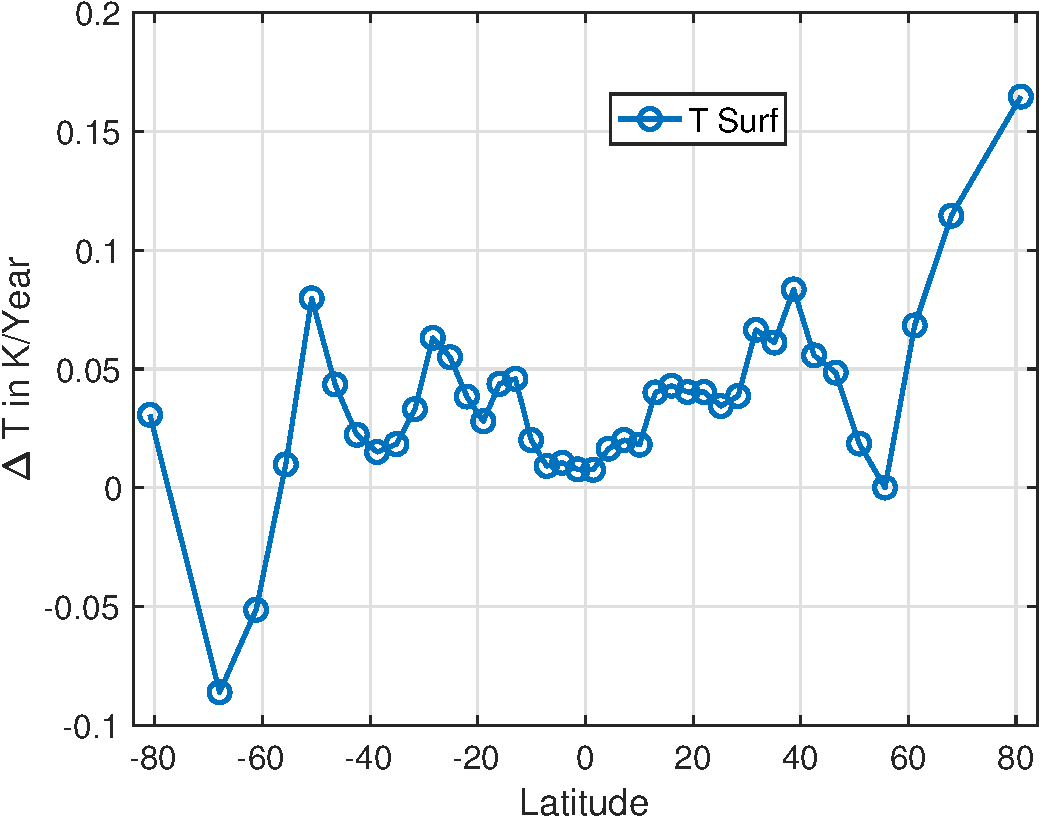
\includegraphics[width=0.8\linewidth]{./Figs/Pdf/tsurf_trend.pdf}
\end{center}
\end{block}
\end{column}

\begin{column}{0.55\columnwidth}
\begin{block}{\footnotesize}
\vspace{-0.1in}
\footnotesize
\begin{itemize}
\item Tropospheric warming, stratospheric cooling
\item Very high arctic warming (as expected)
\item Cloud problems \textpm{} 20 Deg lat in troposphere?
\item Error estimates require off-diagonal measurement error covariance
\end{itemize}
\end{block}
\end{column}
\end{columns}
\end{frame}

\begin{frame}[label={sec:org11e0b32}]{Retrieved \ozone, Clouds}
\vspace{-0.35in}

\begin{columns}
\begin{column}{0.55\columnwidth}
\begin{block}{\footnotesize Cloud Trends}
\vspace{-0.1in}
\begin{center}
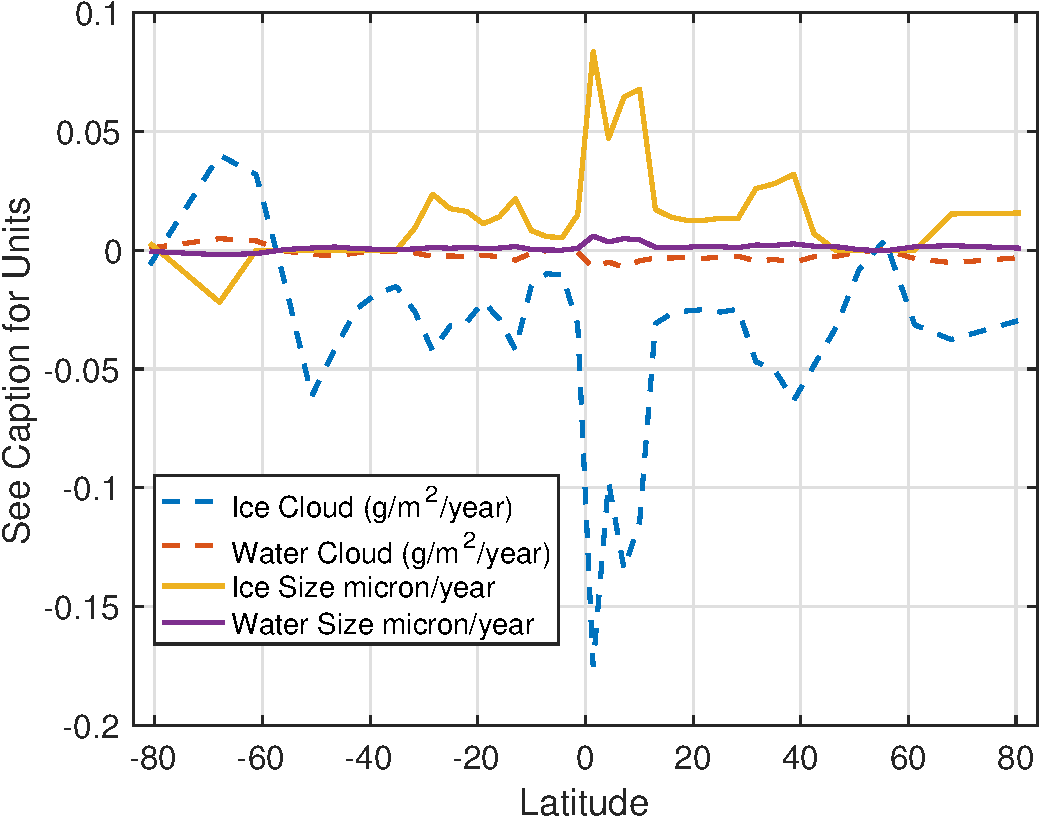
\includegraphics[width=0.9\linewidth]{./Figs/Pdf/cloud_trend.pdf}
\end{center}
\end{block}
\end{column}

\begin{column}{0.55\columnwidth}
\begin{block}{\footnotesize Ozone Trends}
\vspace{-0.1in}
\begin{center}
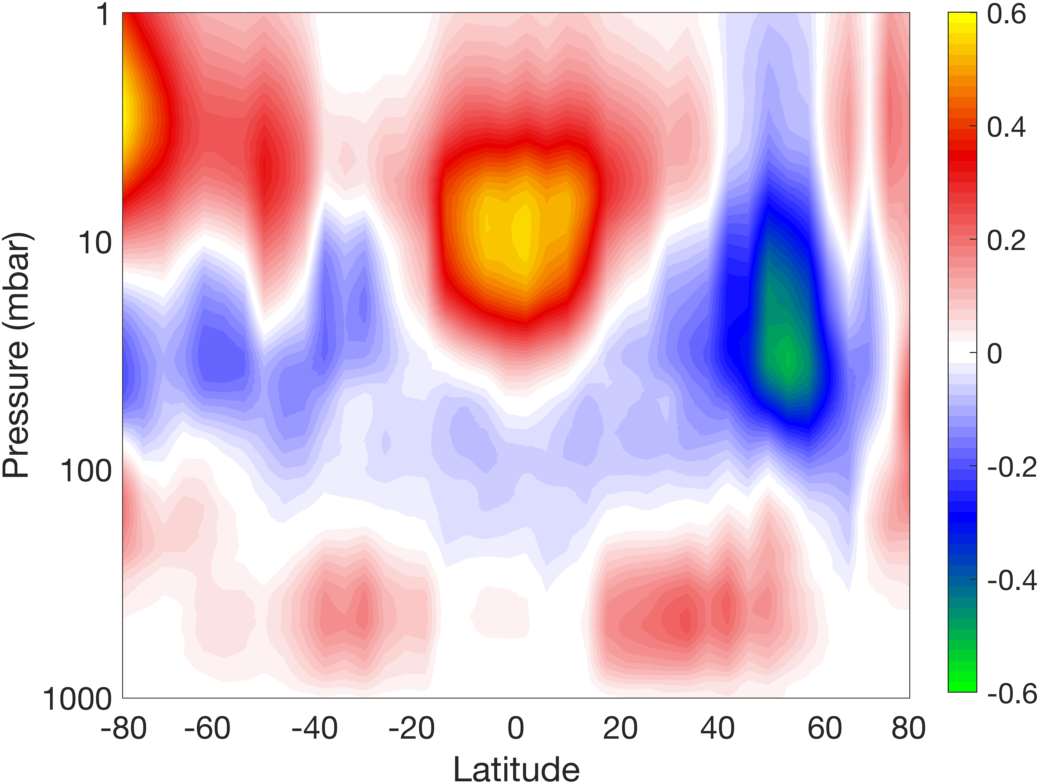
\includegraphics[width=0.9\linewidth]{./Figs/Png/o3_trend_upto_1mbar.png}
\end{center}
\end{block}
\end{column}
\end{columns}


\begin{columns}
\begin{column}{0.55\columnwidth}
\begin{block}{\footnotesize}
\vspace{-0.3in}
\small
\begin{itemize}
\item Ice cloud trends some similarity to B. Kahn's 2018 paper!
\item Except for decrease in ice water path near equator
\end{itemize}
\end{block}
\end{column}

\begin{column}{0.55\columnwidth}
\begin{block}{\footnotesize}
\vspace{-0.3in}
\small
\begin{itemize}
\item Tropospheric \ozone increases similar to the recent literature
\item Stratospheric variability also in agreement, hot topic right now
\end{itemize}
\end{block}
\end{column}
\end{columns}
\end{frame}

\begin{frame}[label={sec:orgca880d6}]{Stratopsheric Ozone Trend Inter-Comparisons}
\vspace{-0.15in}
\begin{block}{\footnotesize Ball et. al., ACP (2018)}
\vspace{-0.1in}
\begin{center}
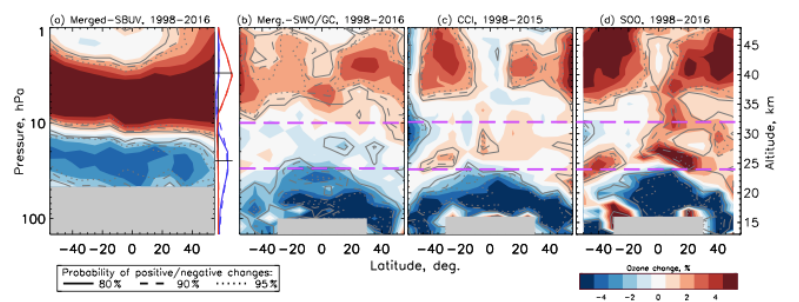
\includegraphics[width=0.9\linewidth]{./Figs/Png/ozone_ball_2018.png}
\end{center}

\vspace{-0.3in}
\end{block}
\begin{columns}
\begin{column}{0.5\columnwidth}
\begin{block}{\footnotesize AIRS Ozone Trends}
\vspace{-0.1in}
\begin{center}
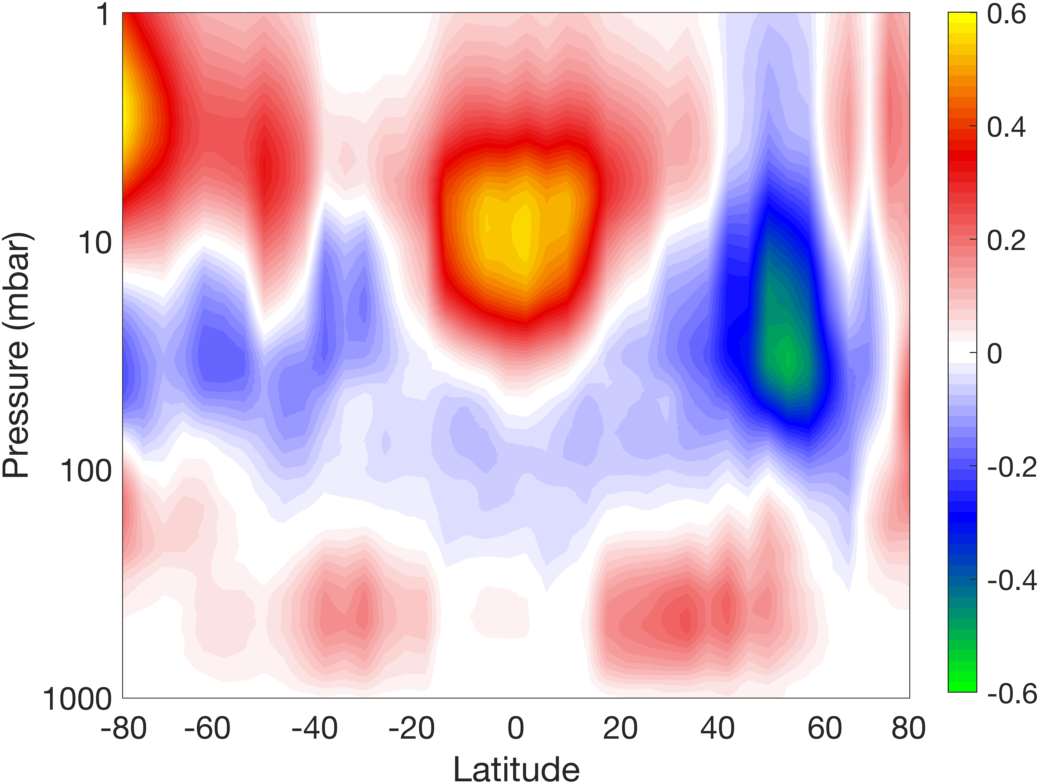
\includegraphics[width=0.85\linewidth]{./Figs/Png/o3_trend_upto_1mbar.png}
\end{center}
\end{block}
\end{column}

\begin{column}{0.55\columnwidth}
\begin{block}{\footnotesize}
\vspace{-0.1in}
\footnotesize
\begin{itemize}
\item We see a nominal 10-100 hPa reduction in \ozone (Chinese CFC issue?)
\item And, somewhat similar increase in \ozone in the upper strat
\item Encouraging results for first look
\end{itemize}
\end{block}
\end{column}
\end{columns}
\end{frame}

\begin{frame}[shrink=10,label={sec:orgcfa8e1d}]{Trend Uncertainties: Only Diagonal Meas. Error Covariance}
\vspace{-0.1in}
\small

\begin{itemize}
\item Trend retrieval \emph{measurement errors} are (a) inter-annual variability (b) instrument drift, and (c) sampling noise

\item Off-diagonal elements of (a) are LARGE and have not been used/characterized, thus error estimates are incorrect.  Trial covariance matrices have large condition numbers.

\item However, uncertainties using diagonal only errors do show reasonable patterns

\item Striping in tropical troposphere likely related to clouds
\end{itemize}

\vspace{-0.1in}

\begin{columns}
\begin{column}{0.55\columnwidth}
\begin{block}{\footnotesize Temperature Uncertainties}
\vspace{-0.1in}
\begin{center}
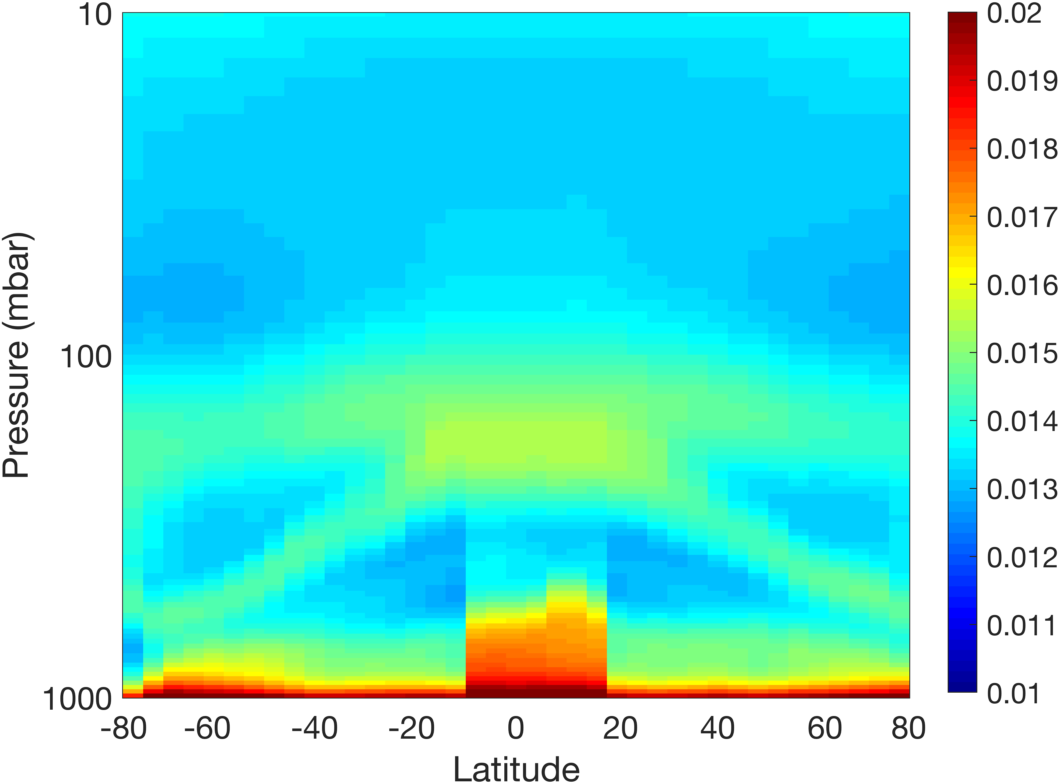
\includegraphics[width=0.9\linewidth]{./Figs/Png/temp_unc.png}
\end{center}
\end{block}
\end{column}

\begin{column}{0.55\columnwidth}
\begin{block}{\footnotesize Water Uncertanties}
\vspace{-0.1in}
\begin{center}
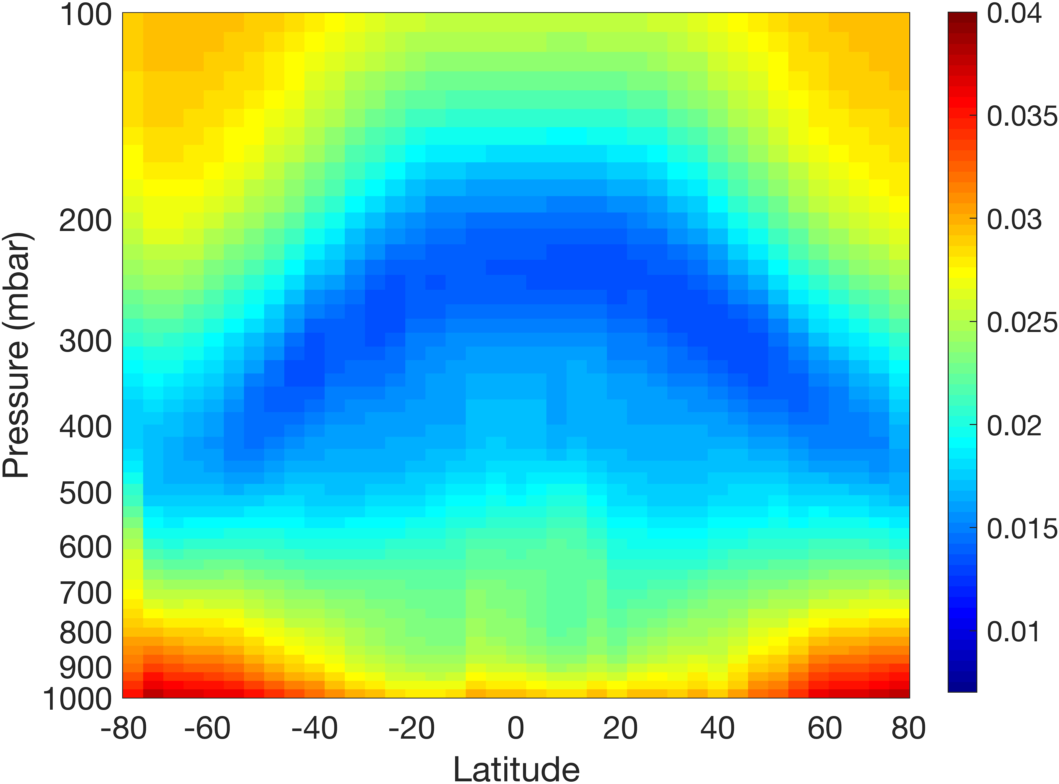
\includegraphics[width=0.9\linewidth]{./Figs/Png/wat_unc.png}
\end{center}
\end{block}
\end{column}
\end{columns}
\end{frame}

\begin{frame}[label={sec:org0133b30}]{Anomaly Example: Water Vapor (27N to 30N Latitude Zonal)}
\vspace{-0.35in}

\begin{columns}
\begin{column}{0.55\columnwidth}
\begin{block}{\footnotesize This work}
\vspace{-0.1in}
\begin{center}
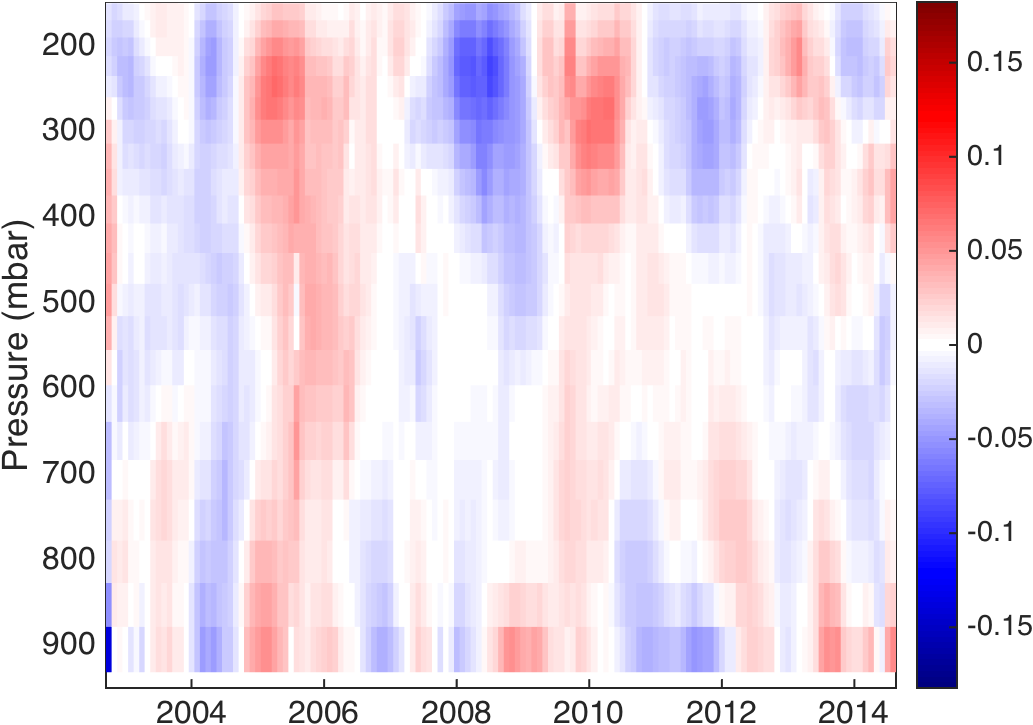
\includegraphics[width=0.8\linewidth]{./oFigs/water_lati_30_UMBC.png}
\end{center}
\end{block}
\end{column}

\begin{column}{0.55\columnwidth}
\begin{block}{\footnotesize ERA \(\times\) Avg Kernel}
\vspace{-0.1in}
\begin{center}
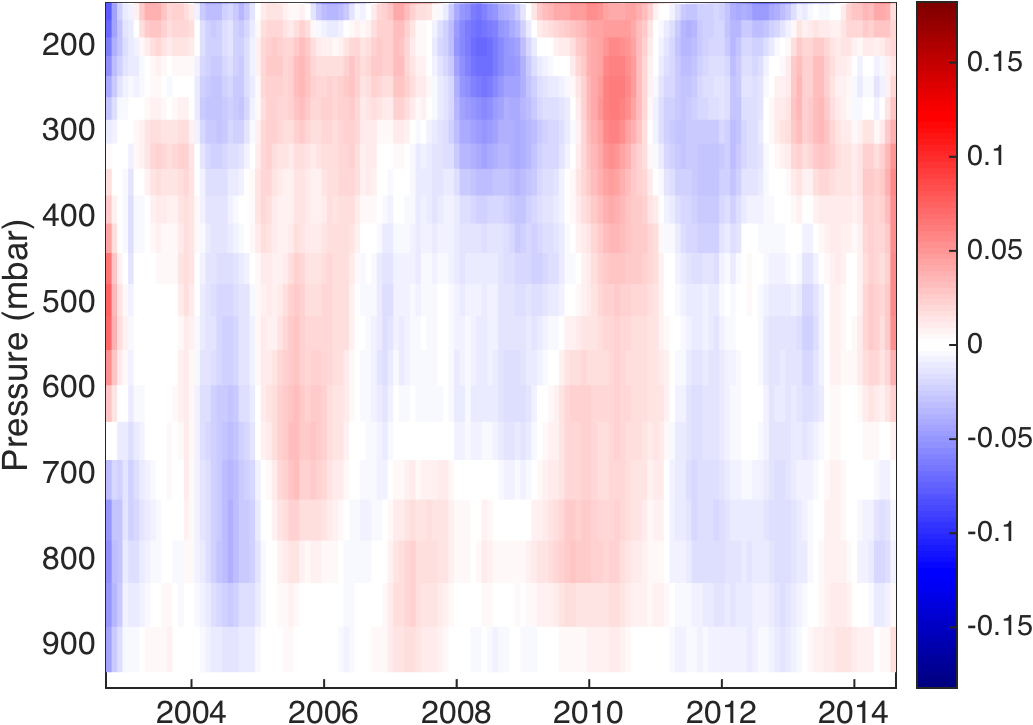
\includegraphics[width=0.8\linewidth]{./oFigs/water_lati_30_ERA.png}
\end{center}
\end{block}
\end{column}
\end{columns}

\vspace{-0.15in}
\begin{columns}
\begin{column}{0.55\columnwidth}
\begin{block}{\footnotesize AIRS Level 3}
\vspace{-0.1in}
\begin{center}
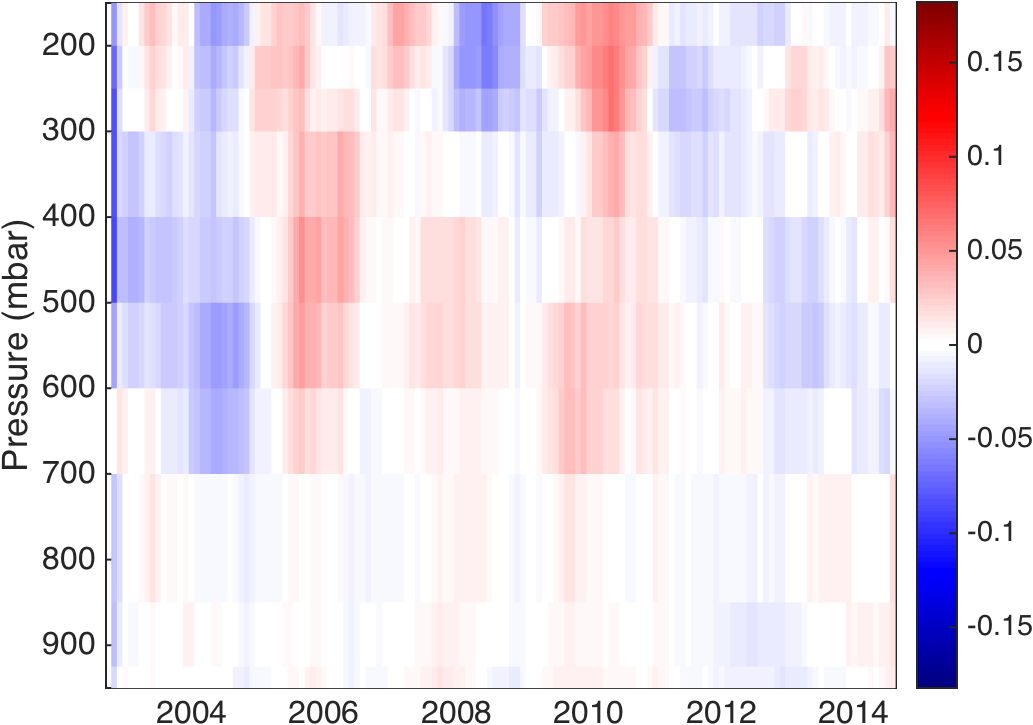
\includegraphics[width=0.8\linewidth]{./oFigs/water_lati_30_L3.png}
\end{center}
\end{block}
\end{column}

\begin{column}{0.55\columnwidth}
\begin{block}{\footnotesize}
\small
\begin{itemize}
\item Input: radiance anomalies, a-priori of zero
\item These are old, working on updates
\item New work using Jacobians that vary with time, here just using a single Jacobian for all times
\end{itemize}
\end{block}
\end{column}
\end{columns}
\end{frame}

\begin{frame}[label={sec:orga4b2b8a}]{Conclusions and Future Work}
\begin{itemize}
\item Develop gridded radiance product using CHIRP data
\item Refine and validate trend and anomaly geophysical products derived from these radiance grids (zonal for now)
\begin{itemize}
\item Measurement error covariances
\item Test TwoSlab cloud approach in more detail
\item Include microwave in trend/anomaly retrievals?
\item Validate, esp. using GPS-RO
\item Retrieve \cd and other minor gases (trends and anomalies)
\end{itemize}
\end{itemize}
\end{frame}
\end{document}